% Created by tikzDevice version 0.12.6 on 2024-02-14 14:51:03
% !TEX encoding = UTF-8 Unicode
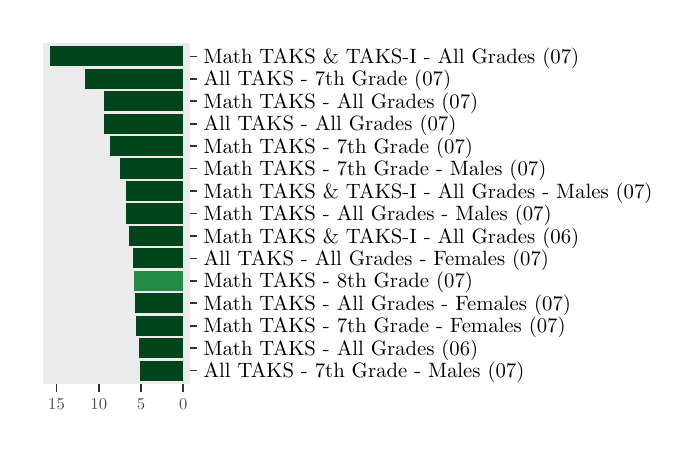
\begin{tikzpicture}[x=1pt,y=1pt]
\definecolor{fillColor}{RGB}{255,255,255}
\path[use as bounding box,fill=fillColor,fill opacity=0.00] (0,0) rectangle (231.26,144.54);
\begin{scope}
\path[clip] (  0.00,  0.00) rectangle (231.26,144.54);
\definecolor{drawColor}{RGB}{255,255,255}
\definecolor{fillColor}{RGB}{255,255,255}

\path[draw=drawColor,line width= 0.6pt,line join=round,line cap=round,fill=fillColor] (  0.00,  0.00) rectangle (231.26,144.54);
\end{scope}
\begin{scope}
\path[clip] (  5.50, 15.75) rectangle ( 58.61,139.04);
\definecolor{fillColor}{gray}{0.92}

\path[fill=fillColor] (  5.50, 15.75) rectangle ( 58.61,139.04);
\definecolor{fillColor}{RGB}{0,68,27}

\path[fill=fillColor] (  7.91,130.52) rectangle ( 56.20,137.82);

\path[fill=fillColor] ( 20.75,122.41) rectangle ( 56.20,129.71);

\path[fill=fillColor] ( 27.69,114.30) rectangle ( 56.20,121.60);

\path[fill=fillColor] ( 27.70,106.19) rectangle ( 56.20,113.49);

\path[fill=fillColor] ( 29.86, 98.08) rectangle ( 56.20,105.38);

\path[fill=fillColor] ( 33.53, 89.97) rectangle ( 56.20, 97.27);

\path[fill=fillColor] ( 35.59, 81.86) rectangle ( 56.20, 89.16);

\path[fill=fillColor] ( 35.61, 73.74) rectangle ( 56.20, 81.04);

\path[fill=fillColor] ( 36.75, 65.63) rectangle ( 56.20, 72.93);

\path[fill=fillColor] ( 37.99, 57.52) rectangle ( 56.20, 64.82);
\definecolor{fillColor}{RGB}{35,139,69}

\path[fill=fillColor] ( 38.37, 49.41) rectangle ( 56.20, 56.71);
\definecolor{fillColor}{RGB}{0,68,27}

\path[fill=fillColor] ( 38.66, 41.30) rectangle ( 56.20, 48.60);

\path[fill=fillColor] ( 39.26, 33.19) rectangle ( 56.20, 40.49);

\path[fill=fillColor] ( 40.10, 25.08) rectangle ( 56.20, 32.38);

\path[fill=fillColor] ( 40.50, 16.97) rectangle ( 56.20, 24.27);
\end{scope}
\begin{scope}
\path[clip] (  0.00,  0.00) rectangle (231.26,144.54);
\definecolor{drawColor}{gray}{0.20}

\path[draw=drawColor,line width= 0.6pt,line join=round] ( 58.61, 20.62) --
	( 61.36, 20.62);

\path[draw=drawColor,line width= 0.6pt,line join=round] ( 58.61, 28.73) --
	( 61.36, 28.73);

\path[draw=drawColor,line width= 0.6pt,line join=round] ( 58.61, 36.84) --
	( 61.36, 36.84);

\path[draw=drawColor,line width= 0.6pt,line join=round] ( 58.61, 44.95) --
	( 61.36, 44.95);

\path[draw=drawColor,line width= 0.6pt,line join=round] ( 58.61, 53.06) --
	( 61.36, 53.06);

\path[draw=drawColor,line width= 0.6pt,line join=round] ( 58.61, 61.17) --
	( 61.36, 61.17);

\path[draw=drawColor,line width= 0.6pt,line join=round] ( 58.61, 69.28) --
	( 61.36, 69.28);

\path[draw=drawColor,line width= 0.6pt,line join=round] ( 58.61, 77.39) --
	( 61.36, 77.39);

\path[draw=drawColor,line width= 0.6pt,line join=round] ( 58.61, 85.51) --
	( 61.36, 85.51);

\path[draw=drawColor,line width= 0.6pt,line join=round] ( 58.61, 93.62) --
	( 61.36, 93.62);

\path[draw=drawColor,line width= 0.6pt,line join=round] ( 58.61,101.73) --
	( 61.36,101.73);

\path[draw=drawColor,line width= 0.6pt,line join=round] ( 58.61,109.84) --
	( 61.36,109.84);

\path[draw=drawColor,line width= 0.6pt,line join=round] ( 58.61,117.95) --
	( 61.36,117.95);

\path[draw=drawColor,line width= 0.6pt,line join=round] ( 58.61,126.06) --
	( 61.36,126.06);

\path[draw=drawColor,line width= 0.6pt,line join=round] ( 58.61,134.17) --
	( 61.36,134.17);
\end{scope}
\begin{scope}
\path[clip] (  0.00,  0.00) rectangle (231.26,144.54);
\definecolor{drawColor}{RGB}{0,0,0}

\node[text=drawColor,anchor=base west,inner sep=0pt, outer sep=0pt, scale=  0.75] at ( 63.56, 18.03) {All TAKS - 7th Grade - Males (07)};

\node[text=drawColor,anchor=base west,inner sep=0pt, outer sep=0pt, scale=  0.75] at ( 63.56, 26.14) {Math TAKS - All Grades (06)};

\node[text=drawColor,anchor=base west,inner sep=0pt, outer sep=0pt, scale=  0.75] at ( 63.56, 34.26) {Math TAKS - 7th Grade - Females (07)};

\node[text=drawColor,anchor=base west,inner sep=0pt, outer sep=0pt, scale=  0.75] at ( 63.56, 42.37) {Math TAKS - All Grades - Females (07)};

\node[text=drawColor,anchor=base west,inner sep=0pt, outer sep=0pt, scale=  0.75] at ( 63.56, 50.48) {Math TAKS - 8th Grade (07)};

\node[text=drawColor,anchor=base west,inner sep=0pt, outer sep=0pt, scale=  0.75] at ( 63.56, 58.59) {All TAKS - All Grades - Females (07)};

\node[text=drawColor,anchor=base west,inner sep=0pt, outer sep=0pt, scale=  0.75] at ( 63.56, 66.70) {Math TAKS \& TAKS-I - All Grades (06)};

\node[text=drawColor,anchor=base west,inner sep=0pt, outer sep=0pt, scale=  0.75] at ( 63.56, 74.81) {Math TAKS - All Grades - Males (07)};

\node[text=drawColor,anchor=base west,inner sep=0pt, outer sep=0pt, scale=  0.75] at ( 63.56, 82.92) {Math TAKS \& TAKS-I - All Grades - Males (07)};

\node[text=drawColor,anchor=base west,inner sep=0pt, outer sep=0pt, scale=  0.75] at ( 63.56, 91.03) {Math TAKS - 7th Grade - Males (07)};

\node[text=drawColor,anchor=base west,inner sep=0pt, outer sep=0pt, scale=  0.75] at ( 63.56, 99.15) {Math TAKS - 7th Grade (07)};

\node[text=drawColor,anchor=base west,inner sep=0pt, outer sep=0pt, scale=  0.75] at ( 63.56,107.26) {All TAKS - All Grades (07)};

\node[text=drawColor,anchor=base west,inner sep=0pt, outer sep=0pt, scale=  0.75] at ( 63.56,115.37) {Math TAKS - All Grades (07)};

\node[text=drawColor,anchor=base west,inner sep=0pt, outer sep=0pt, scale=  0.75] at ( 63.56,123.48) {All TAKS - 7th Grade (07)};

\node[text=drawColor,anchor=base west,inner sep=0pt, outer sep=0pt, scale=  0.75] at ( 63.56,131.59) {Math TAKS \& TAKS-I - All Grades (07)};
\end{scope}
\begin{scope}
\path[clip] (  0.00,  0.00) rectangle (231.26,144.54);
\definecolor{drawColor}{gray}{0.20}

\path[draw=drawColor,line width= 0.6pt,line join=round] ( 56.20, 13.00) --
	( 56.20, 15.75);

\path[draw=drawColor,line width= 0.6pt,line join=round] ( 40.94, 13.00) --
	( 40.94, 15.75);

\path[draw=drawColor,line width= 0.6pt,line join=round] ( 25.69, 13.00) --
	( 25.69, 15.75);

\path[draw=drawColor,line width= 0.6pt,line join=round] ( 10.43, 13.00) --
	( 10.43, 15.75);
\end{scope}
\begin{scope}
\path[clip] (  0.00,  0.00) rectangle (231.26,144.54);
\definecolor{drawColor}{gray}{0.30}

\node[text=drawColor,anchor=base,inner sep=0pt, outer sep=0pt, scale=  0.60] at ( 56.20,  6.67) {0};

\node[text=drawColor,anchor=base,inner sep=0pt, outer sep=0pt, scale=  0.60] at ( 40.94,  6.67) {5};

\node[text=drawColor,anchor=base,inner sep=0pt, outer sep=0pt, scale=  0.60] at ( 25.69,  6.67) {10};

\node[text=drawColor,anchor=base,inner sep=0pt, outer sep=0pt, scale=  0.60] at ( 10.43,  6.67) {15};
\end{scope}
\end{tikzpicture}
